\documentclass[12pt]{article}%
\usepackage{amsfonts}
\usepackage{fancyhdr}
\usepackage{comment}
\usepackage[a4paper, top=2.5cm, bottom=2.5cm, left=2.2cm, right=2.2cm]%
{geometry}
\usepackage{times}
\usepackage{amsmath}
\usepackage{changepage}
\usepackage{amssymb}
\usepackage{graphicx}%
%table
\usepackage{tabu}
\usepackage{booktabs}
\usepackage{threeparttable}
\usepackage{multirow}



\setcounter{MaxMatrixCols}{30}
\newtheorem{theorem}{Theorem}
\newtheorem{acknowledgement}[theorem]{Acknowledgement}
\newtheorem{algorithm}[theorem]{Algorithm}
\newtheorem{axiom}{Axiom}
\newtheorem{case}[theorem]{Case}
\newtheorem{claim}[theorem]{Claim}
\newtheorem{conclusion}[theorem]{Conclusion}
\newtheorem{condition}[theorem]{Condition}
\newtheorem{conjecture}[theorem]{Conjecture}
\newtheorem{corollary}[theorem]{Corollary}
\newtheorem{criterion}[theorem]{Criterion}
\newtheorem{definition}[theorem]{Definition}
\newtheorem{example}[theorem]{Example}
\newtheorem{exercise}[theorem]{Exercise}
\newtheorem{lemma}[theorem]{Lemma}
\newtheorem{notation}[theorem]{Notation}
\newtheorem{problem}[theorem]{Problem}
\newtheorem{proposition}[theorem]{Proposition}
\newtheorem{remark}[theorem]{Remark}
\newtheorem{solution}[theorem]{Solution}
\newtheorem{summary}[theorem]{Summary}
\newenvironment{proof}[1][Proof]{\textbf{#1.} }{\ \rule{0.5em}{0.5em}}

\newcommand{\Q}{\mathbb{Q}}
\newcommand{\R}{\mathbb{R}}
\newcommand{\C}{\mathbb{C}}
\newcommand{\Z}{\mathbb{Z}}

\begin{document}

\title{Markov Decision Processes-Homework3}
\author{Xiongming Dai}
\date{November 20,2017}
\maketitle
\section{Questions}

    (1) We assume that X  denotes the number of days since the last repair or maintenance. As the problems states, the system fails with probability 1 sometime during the 30th day if the system continues for 30 days without repair or maintenance. Hence, 

\begin{align}
  & state=d+1,d=0,1,...,30. \\ 
 & state\in (1,31) 
\end{align}

The actions in the Markov Decision Processes are Produce and Maintain:\\
 $Actions=\{Produce,Maintain\}$.
The system will fail on the $d$th day since the last repair or maintenance with probability of failure of 
$(1-{{\psi }^{d}}),$ The transition probability matrix of action "Produce" can be written as:

\[TP{{M}_{\Pr oduce}}=\left[ \begin{matrix}
   0 & 1 & 0 & ... & 0 & ... & 0 & 0  \\
   1-\psi  & 0 & \psi  & 0 & 0 & ... & 0 & 0  \\
   1-{{\psi }^{2}} & 0 & 0 & {{\psi }^{2}} & 0 & ... & 0 & 0  \\
   \vdots  & {} & {} & {} & {} & {} & {} & {}  \\
   1-{{\psi }^{d}} & 0 & ... & ... & 0 & {{\psi }^{d}} & ... & 0  \\
   \vdots  & {} & {} & {} & {} & {} & {} & {}  \\
   1-{{\psi }^{29}} & 0 & ... & 0 & ... & 0 & 0 & {{\psi }^{29}}  \\
   1 & 0 & ... & 0 & ... & 0 & 0 & 0  \\
\end{matrix} \right]\]

Where $d=1,2,...,29.$

Since the cost of repair is $\$450$ , so reward is -450, we can formulate the transition reward matrix given the action "Produce" as:

\[TR{{M}_{\Pr oduce}}=\left[ \begin{matrix}
   0 & 0 & 0 & ... & 0 & ... & 0 & 0  \\
   -450 & 0 & 0 & 0 & 0 & ... & 0 & 0  \\
   -450 & 0 & 0 & 0 & 0 & ... & 0 & 0  \\
   \vdots  & {} & {} & {} & {} & {} & {} & {}  \\
   -450 & 0 & ... & ... & 0 & 0 & ... & 0  \\
   \vdots  & {} & {} & {} & {} & {} & {} & {}  \\
   -450 & 0 & ... & 0 & ... & 0 & 0 & 0  \\
   -450 & 0 & ... & 0 & ... & 0 & 0 & 0  \\
\end{matrix} \right]\]

The TPM and TRM given action "Produce" are the matrix with the size of $31 \times 31$.

From the statement that after the system is repaired or maintained, it is assumed to be as good as new. It means that that machine will go to state 0 every time after maintenance. Therefore, the transition probability matrix of action "Maintain" could be written as:

\[TP{{M}_{Ma\operatorname{int}ain}}=\left[ \begin{matrix}
   0 & 0 & 0 & ... & 0 & ... & 0 & 0  \\
   1 & 0 & 0 & 0 & 0 & ... & 0 & 0  \\
   1 & 0 & 0 & 0 & 0 & ... & 0 & 0  \\
   \vdots  & {} & {} & {} & {} & {} & {} & {}  \\
   1 & 0 & ... & ... & 0 & 0 & ... & 0  \\
   \vdots  & {} & {} & {} & {} & {} & {} & {}  \\
   1 & 0 & ... & 0 & ... & 0 & 0 & 0  \\
   1 & 0 & ... & 0 & ... & 0 & 0 & 0  \\
\end{matrix} \right]\]

The cost for maintenance is $\$175$, so reward is -175, similarly, we can formulate the transition reward matrix given the action "Maintain" as:

\[TR{{M}_{Ma\operatorname{int}ain}}=\left[ \begin{matrix}
   0 & 0 & 0 & ... & 0 & ... & 0 & 0  \\
   -175 & 0 & 0 & 0 & 0 & ... & 0 & 0  \\
   -175 & 0 & 0 & 0 & 0 & ... & 0 & 0  \\
   \vdots  & {} & {} & {} & {} & {} & {} & {}  \\
   -175 & 0 & ... & ... & 0 & 0 & ... & 0  \\
   \vdots  & {} & {} & {} & {} & {} & {} & {}  \\
   -175 & 0 & ... & 0 & ... & 0 & 0 & 0  \\
   -175 & 0 & ... & 0 & ... & 0 & 0 & 0  \\
\end{matrix} \right]\]

The mapping structure can be descriped in Figure 1.

\begin{figure*}
\begin{center}
%\fbox{\rule{0pt}{2in} \rule{.9\linewidth}{0pt}}
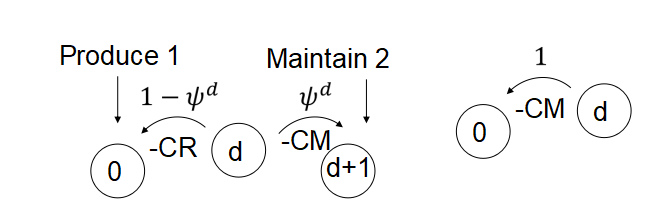
\includegraphics[width=0.8\linewidth]{map.jpg}
\end{center}
   \caption{Roughly description about the MDP}
\label{fig:short}
\end{figure*}


(2) In order to identify the optimal policy for the manager, the code using relative value iteration for average reward is shown as follows:\\

$"main\_HW3\_Problem1\_Dai.m"$ , which  is the main function that shows the optimal policy and its iteration record.\\
$"func\_HW3\_Problem\_1\_RVI.m"$ is an self-defined function for conducting relative value iteration. \\

If you want to know the whole process of my code, please run the the main function file, and you will find the result, simultaneously, the output will be stored into the file(diary.txt) with comand "diary on" and "diary off".

\begin{figure*}
\begin{center}
%\fbox{\rule{0pt}{2in} \rule{.9\linewidth}{0pt}}
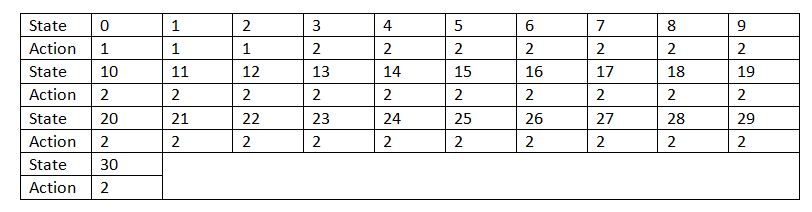
\includegraphics[width=0.8\linewidth]{record.jpg}
\end{center}
   \caption{Record about the states associated the actions}
\label{fig:short}
\end{figure*}





(3) Please Note that $\varepsilon =0.01$ , and the maximization number of iterations is 500 . The  optimal policy for $\psi =0.9$ is shown in Figure 2.  the action "1" represents "Produce", and action "2" represents "Maintain".

The results show that the optimal policy for preventative maintenance of the machine is the machine should be maintained after 2 days since the last repair or maintenance.

\section{Questions}

The TPM associated with action a is $P_a$ and the associated TRM is $R_a$.

\begin{align}
  & {{P}_{1}}=\left[ \begin{matrix}
   0.1 & 0.9  \\
   0.8 & 0.2  \\
\end{matrix} \right],{{R}_{1}}=\left[ \begin{matrix}
   12 & 16  \\
   -7 & 13  \\
\end{matrix} \right]
 & {{P}_{2}}=\left[ \begin{matrix}
   0.3 & 0.7  \\
   0.5 & 0.5  \\
\end{matrix} \right],{{R}_{2}}=\left[ \begin{matrix}
   12 & -11  \\
   6 & 9  \\
\end{matrix} \right] 
\end{align}

The state(action) trajectory is: 
$1(1),2(2),1(2),2(2),2(X)$. And we have known that the system starts at state 1.

$\bf{State 1}$. Set all the Q-factors to 0:
$Q(1,1)=Q(1,2)=Q(2,1)=Q(2,2)=0$
The set of actions allowed in state 1 is $A(1)=\{1,2\}$ and that allowed in state 2 is $A(2)=\{1,2\}$. Clearly $|A(i)|=2,i=1,2$. Let the step size $\alpha $ be defined by $\alpha =\frac{10}{20+k}$. select an action with probability $\frac{1}{|A(i)|}$. Let the selected action be 1. simulate action 1. Let the next state be 2.

$\bf{State 2}$.The current state (j) is 2 and the old state (i) was 1. The action (a) selected in the old state was 1. So we now have to update Q(1,1). Now:k=0, $\alpha=0.5$;

\begin{align}
  & r(i,a,j)=r(1,1,2)=16 \\ 
 & \underset{b}{\mathop{\max }}\,Q(j,b)=\underset{b}{\mathop{\max }}\,Q(2,b)=\max \{Q(2,1),Q(2,2)\}=0; \\
  & Q(1,1)\leftarrow (1-\alpha )Q(1,1)+\alpha [r(1,1,2)+\lambda \underset{b\in A(2)}{\mathop{\max }}\,Q(2,b)] \\ 
 & =0.5*0+0.5*(16+0.7*0)=8 
\end{align}

Current state is 2 and the selected action is 2. Simulate action 2. Let the next state be 1.

$\bf{State 1(again)}$ The current state(j) is 1 and the old state (i) was 2. The action(a) selected in the old state was 2. So we now have to update Q(2,2). Now:k=1;$\alpha=10/21$.

\begin{align}
  & r(i,a,j)=r(2,2,1)=6 \\ 
 & \underset{b}{\mathop{\max }}\,Q(1,b)=\underset{b}{\mathop{\max }}\,Q(1,b)=\max \{Q(1,1),Q(1,2)\}=\max \{8,0\}=8; \\ 
 & Q(2,2)\leftarrow (1-\alpha )Q(2,2)+\alpha [r(2,2,1)+\lambda \underset{b\in A(1)}{\mathop{\max }}\,Q(1,b)] \\ 
 & =\frac{11}{21}*0+\frac{10}{21}*(6+0.7*8)=5.5238 
\end{align}

Current state is 1 and the selected action is 2. Simulate action 2 and the next state is 2.

$\bf{State 2(again)}$  The current state(j) is 2 and the old state(i) was 1. The action(a) selected in the old state was 2. We we now have to update Q(1,2). Now: k=2;$\alpha=5/11$.

\begin{align}
  & r(i,a,j)=r(1,2,2)=-11 \\ 
 & \underset{b}{\mathop{\max }}\,Q(2,b)=\underset{b}{\mathop{\max }}\,Q(2,b)=\max \{Q(2,1),Q(2,2)\}=\max \{0,5.5238\}=5.5238; \\ 
 & Q(1,2)\leftarrow (1-\alpha )Q(1,2)+\alpha [r(1,2,2)+\lambda \underset{b\in A(2)}{\mathop{\max }}\,Q(2,b)] \\ 
 & =\frac{6}{11}*0+\frac{5}{11}*(-11+0.7*5.5238)=-3.2424 
\end{align}

Current state is 2 and the selected action is 2. Simulate action 2 and the next state is 2.

$\bf{State 2(a\ \ third \ \ time)}$  The current state(j) is 2 and the old state(i) was 2. The action(a) selected in the old state was 2. We we now have to update Q(2,2). Now: k=3;$\alpha=10/23$.

\begin{align}
  & r(i,a,j)=r(2,2,2)=9 \\ 
 & \underset{b}{\mathop{\max }}\,Q(2,b)=\underset{b}{\mathop{\max }}\,Q(2,b)=\max \{Q(2,1),Q(2,2)\}=\max \{0,5.5238\}=5.5238; \\ 
 & Q(2,2)\leftarrow (1-\alpha )Q(2,2)+\alpha [r(2,2,2)+\lambda \underset{b\in A(2)}{\mathop{\max }}\,Q(2,b)] \\ 
 & =\frac{13}{23}*5.5238+\frac{10}{23}*(9+0.7*5.5238)=8.7163 
\end{align}

Current state is 2 and the selected action is X. 


























 
  
  
  
  
  
  




\end{document}